% ============================================================
% APPENDIX C -- Disease-Specific Example: Haemophilia
% Rewritten to mirror Appendix A: Purpose -> Definitions ->
% Specialisation mapping -> Propositions -> Proofs -> Simulations -> Summary.
% ============================================================

\label{app:hemo_dynamics}

\begin{ataglance}[How to read this appendix]
This is Mr~B's appendix. Appendix~\ref{app:dynamical} built a
disease-independent machine; here the abstract symbols are given names a
haematologist uses. The latent state $X$ becomes circulating factor~VIII or
IX activity, the inhibitory factor $Y$ becomes inhibitor titre in Bethesda
units, and and, for haemophilia~A, the homeostatic factor $Z$ becomes von~Willebrand
factor. Von~Willebrand factor stabilises factor~VIII and not factor~IX, so in
haemophilia~B the stabilisation term $h(Z)$ is set to zero and the model
reduces to infusion, neutralisation and clearance.

Four questions are asked in order. What governs factor activity moment to
moment (\S\ref{sec:C_definitions})? Where does it settle, and at what inhibitor
titre does the settling point fall below the level that prevents bleeding
(\S\ref{sec:C_kinetics})? What do immune tolerance induction and gene therapy do
to those equations (\S\ref{sec:C_therapy})? And what happens when the whole
thing is simulated with noise (\S\ref{sec:C_simulation})?

The results are illustrative. No patient data are used and nothing here forms
part of the validation in the main text. The value of the exercise is that it
turns clinical intuitions about inhibitors, which are usually expressed as rules
of thumb, into statements that could be wrong.
\end{ataglance}

\section{Purpose and Scope}
\label{sec:C_purpose}
Appendix~\ref{app:dynamical} introduced a disease-independent mathematical
framework. This appendix demonstrates how that framework specialises to a
clinically relevant disease, haemophilia. The purpose is illustrative rather
than empirical: the specifications show how the general ODE--SDE--PDE
architecture represents clotting-factor kinetics, inhibitor development, immune
tolerance induction, and gene therapy \citep{nathwani_2011}, and the numerical outputs come from
simulation, not patient data. Nothing here is part of the validation in the main
text.

Before any of it can be written down, the abstract symbols of
Appendix~\ref{app:dynamical} have to be given haematological names.

\section{Relationship to the General Framework}
\label{sec:C_relationship}
The present appendix specialises the disease-independent framework of
Appendix~\ref{app:dynamical}: the abstract state $X$ becomes circulating factor
activity $S_T$, the inhibitory factor $Y$ becomes inhibitor titre, and the
homeostatic factor $Z$ becomes von Willebrand factor. The mathematical
definitions of the conceptual variables remain those of
Appendix~\ref{app:mathematical_foundations}, and the computational realisation is
Appendix~\ref{app:computation}. Each proposition below carries the name of the
test that asserts it, in
\texttt{verification/tests/test\_haemophilia.py}; the outcome of running them is
in Appendix~\ref{app:verification}.

The substitution is set out next, one variable at a time, so that a clinician
can check whether each abstract object has been given a sensible clinical
reading.

\section{Definitions and Specialisation Mapping}
\label{sec:C_definitions}

\begin{definition}[Clotting-factor state]
\label{def:C_state}
Let $S_T(t)$ (IU/dL) denote circulating factor~VIII or IX activity, $Y(t)$ (BU)
the inhibitor titre, and $Z$ the von Willebrand factor concentration. The
specialised model maps \eqref{eq:B_ode} onto Michaelis--Menten and Hill kinetics
\citep{michaelis_menten_1913,hill_1910}:
\begin{equation}
\frac{dS_T}{dt}=\underbrace{\frac{V_{\max}T}{K_m+T}}_{\text{infusion }f(T)}
-\underbrace{\alpha S_T\frac{Y^\beta}{K_I^\beta+Y^\beta}}_{\text{neutralisation }g(Y,S_T)}
+\underbrace{\gamma\frac{Z^n}{K_h^n+Z^n}}_{\text{VWF stabilisation }h(Z)}
-\lambda S_T,
\label{eq:C_ode}
\end{equation}
with clearance rate $\lambda$. The Hill exponent $\beta>1$ gives threshold-like
escalation of neutralisation once $Y$ exceeds $K_I$; $n$ captures cooperative
FVIII--VWF binding.
\end{definition}

\begin{reading}[Equation \eqref{eq:C_ode}, term by term]
Read the right-hand side as a ledger of everything that raises or lowers
circulating factor activity in the next instant.

\textbf{$V_{\max}T/(K_m+T)$, infusion.} Michaelis--Menten saturation. Doubling
the infused dose $T$ does not double the rise in activity once $T$ is well
above $K_m$; the curve flattens. Clinically this is the familiar diminishing
return on very large doses, and it is why dosing is repeated rather than simply
enlarged.

\textbf{$\alpha S_T Y^\beta/(K_I^\beta+Y^\beta)$, neutralisation.} A Hill term
with exponent $\beta>1$, which is the important choice. A Hill exponent above
one makes the curve sigmoid rather than gradual: neutralisation is negligible
while $Y$ sits below $K_I$, then climbs steeply once it passes. This is the
formal version of what clinicians describe as a patient ``developing an
inhibitor'', which presents as a threshold event rather than a slow drift.

\textbf{$\gamma Z^n/(K_h^n+Z^n)$, von~Willebrand stabilisation.} Factor~VIII
circulates bound to von~Willebrand factor and is cleared quickly without it.
The Hill form with $n>1$ encodes cooperative binding.

\textbf{$-\lambda S_T$, clearance.} First-order elimination, the standard
half-life term.

The whole equation is therefore a one-compartment pharmacokinetic model with
one addition that matters: the elimination term is not constant but is itself
driven by an immune process that has its own dynamics.
\end{reading}

\begin{definition}[Linear reference model]
\label{def:C_linear}
The traditional linearised form is
$dS_T/dt=k_{\text{in}}T-k_{\text{inh}}Y-k_{\text{decay}}S_T$, which assumes
independence and proportionality among input, inhibition, and clearance.
\end{definition}

The linear model is the one implicitly used whenever a recovery and a half-life
are quoted and a dose is calculated from them. It is not wrong; it is a limiting
case, and the first proposition below says exactly which limit. Knowing the
limit is what tells a clinician when the arithmetic on the ward can be trusted
and when it cannot.

\section{Factor Kinetics}
\label{sec:C_kinetics}

\begin{proposition}[Linear approximation]
\label{prop:C_linear}
For small inhibitor titre the Hill neutralisation term reduces to the linear
model: the leading term of $\alpha S_T\,Y^\beta/(K_I^\beta+Y^\beta)$ about $Y=0$
is $\alpha S_T (Y/K_I)^\beta$, which at $\beta=1$ is exactly the linear
neutralisation $\alpha S_T Y/K_I$, so $k_{\text{inh}}=\alpha/K_I$.
\end{proposition}
\begin{proof}
Expanding $Y^\beta/(K_I^\beta+Y^\beta)=(Y/K_I)^\beta[1-(Y/K_I)^\beta+\cdots]$ for
$Y\ll K_I$ leaves the leading term $(Y/K_I)^\beta$; at $\beta=1$ this is
$Y/K_I$, giving the linear coefficient.
\end{proof}

\begin{reading}[When the ward arithmetic is safe]
This proposition is reassurance with a boundary attached. For $Y\ll K_I$, that
is, a patient with a low-titre or absent inhibitor, the non-linear model
collapses to the linear one and the standard dose calculation is correct.

The boundary is $Y$ approaching $K_I$. Above it the linear model does not merely
lose a little accuracy; because $\beta>1$, it understates neutralisation by a
growing factor, and it understates it most at the titres where getting the dose
right matters most.

For Mr~B this is the difference between the years before his inhibitor was
detected, when conventional dosing worked and the linear model would have
predicted it correctly, and the years after, when the same calculation began
producing doses that failed. Nothing about the underlying biology changed at the
moment of detection. What changed was that his $Y$ crossed into the region where
the approximation stops holding.
\end{reading}
\checkedby{tests/test_haemophilia.py::test_proposition_linear_approximation_at_low_titre}

\begin{proposition}[Stability]
\label{prop:C_stability}
For fixed inhibitor titre $Y$, \eqref{eq:C_ode} has the unique stable
equilibrium
$S_T^\ast(Y)=(f+h)/\big(\alpha\,Y^\beta/(K_I^\beta+Y^\beta)+\lambda\big)$,
because the Jacobian $\partial(\dot S_T)/\partial S_T=-(\alpha\,\mathrm{Hill}(Y)+\lambda)<0$.
\end{proposition}
\begin{proof}
Setting $\dot S_T=0$ isolates $S_T^\ast$; the derivative of the right-hand side
in $S_T$ is $-(\alpha\,\mathrm{Hill}(Y)+\lambda)$, negative for all $Y\ge0$, so
the fixed point is asymptotically stable and trajectories from any initial
activity converge to it.
\end{proof}

\begin{reading}[The inhibitor sits in the denominator]
The steady state $S_T^\ast(Y)=(f+h)/(\alpha\,\mathrm{Hill}(Y)+\lambda)$ is again
input over output, but now the output term carries the inhibitor.

The clinical consequence is that the loss is front-loaded. Worked
Example~\ref{ex:apc-steady} puts the numbers on it, and the pattern is that
almost all of the damage is done before the titre reaches $K_I$, after which
the curve flattens because neutralisation is already close to maximal.

Both halves of that pattern matter. The steep early section is why a so-called
low-titre inhibitor is not a minor finding: it has already cut steady-state
activity substantially at unchanged dosing. The flat later section is why
very-high-titre patients gain little from dose escalation, and why bypassing
agents, which act through a different route rather than raising the numerator,
are used instead.
\end{reading}
\checkedby{tests/test_haemophilia.py::test_proposition_steady_state_is_stable_and_decreasing_in_Y}

\begin{workedexample}[apc-steady]{Where the inhibitor does its damage}
Take a regimen with numerator $f+h=60$ arbitrary units, clearance
$\lambda=1.0$, maximal neutralisation $\alpha=4.0$, $K_I=5$~BU and $\beta=2$.
Proposition~\ref{prop:C_stability} gives the steady state at each titre.

\begin{wecode}[Python]
from hpv.haemophilia import steady_state

REG = dict(numerator=60.0, alpha=4.0, K_I=5.0, beta=2.0, lam=1.0)
prev = None
for Y in (0, 1, 2, 3, 5, 10, 15, 40):
    s = steady_state(Y, **REG)
    lost = "" if prev is None else f"  lost since last: {prev - s:6.2f}"
    print(f"Y = {Y:>2} BU   S_T* = {s:6.2f}{lost}")
    prev = s
\end{wecode}

\noindent The run gives $60.00$, $52.00$, $38.67$, $29.14$, $20.00$, $14.29$,
$13.04$ and $12.15$. Group the losses and the shape is plain: the first two
Bethesda units remove $21.3$ units of activity, a third of baseline; the next
three remove $18.7$; the following ten remove $7.0$; and everything above
$15$~BU removes less than $1$.

A clinician reading only the levels sees a curve falling smoothly. A clinician
reading the losses sees that the interval from $0$ to $3$~BU costs more than
the interval from $5$ to $40$~BU, which inverts the usual intuition that a
high-titre inhibitor is the dangerous one. The high-titre patient is in a worse
place; the low-titre patient is on the steep part of the slope.

\weanswer{$S_T^\ast$ falls from $60$ to $38.67$ over the first two Bethesda
units, and by only $7.0$ more over the next ten. Asserted by
\texttt{test\_worked\_example\_where\_the\_damage\_happens}.}
\end{workedexample}

\begin{proposition}[Inhibitor threshold]
\label{prop:C_threshold}
In a high-neutralisation regime there is a finite inhibitor titre $Y_{\text{thr}}$
at which $S_T^\ast(Y)$ falls to the protective threshold $S_{\text{prot}}$:
\[
Y_{\text{thr}}=K_I\left(\frac{h_{\text{need}}}{1-h_{\text{need}}}\right)^{1/\beta},
\qquad h_{\text{need}}=\frac{(f+h)/S_{\text{prot}}-\lambda}{\alpha},
\]
provided $0<h_{\text{need}}<1$; below $Y_{\text{thr}}$, $S_T^\ast>S_{\text{prot}}$,
and above it $S_T^\ast<S_{\text{prot}}$.
\end{proposition}
\begin{proof}
Solve $S_T^\ast(Y)=S_{\text{prot}}$ for the required Hill value $h_{\text{need}}$,
then invert the Hill function \citep{hill_1910} $\mathrm{Hill}(Y)=h_{\text{need}}$ for $Y$. The
monotonicity of $S_T^\ast$ in $Y$ (neutralisation increases with titre) gives the
sign change across $Y_{\text{thr}}$. The lower non-linear steady state relative to
the linear reference is qualitatively consistent with unexpected breakthrough
bleeds at high titre.
\end{proof}

\begin{reading}[$Y_{\text{thr}}$ as a clinical decision point]
This proposition converts a curve into a number a clinic could act on. Given a
regimen and a protective threshold, there is a single inhibitor titre at which
the patient's steady-state activity crosses from adequate to inadequate.

Continue the arithmetic above with a protective threshold of
$S_{\text{prot}}=20$. Then $h_{\text{need}}=(60/20-1.0)/4.0=0.5$, and
$Y_{\text{thr}}=5\left(0.5/0.5\right)^{1/2}=5$~BU. Below $5$~BU this regimen
keeps Mr~B protected; above it, it does not, and no amount of adherence will
change that.

Two things follow. The threshold depends on the regimen, so it moves when the
dose or the product changes, which means it is a property of the
patient-and-treatment pair rather than of the patient. And the crossing is
sharp because $\beta>1$: there is no comfortable margin either side. A patient
observed at $4$~BU and doing well may be a fortnight of anamnestic response away
from a regimen that no longer works, which is the quantitative case for
monitoring titre rather than waiting for a breakthrough bleed to reveal it.
\end{reading}
\checkedby{tests/test_haemophilia.py::test_proposition_inhibitor_threshold}

\begin{workedexample}[apc-threshold]{Buying titre headroom with dose}
The threshold is a property of the patient and the regimen together, so a
clinician can move it. Keep $S_{\text{prot}}=20$ and raise the numerator, which
is what increasing the dose or switching to a higher-recovery product does.

\begin{wecode}[Python]
from hpv.haemophilia import inhibitor_threshold

REG = dict(alpha=4.0, K_I=5.0, beta=2.0, lam=1.0)
for numerator in (60.0, 75.0, 90.0, 110.0):
    try:
        thr = inhibitor_threshold(numerator=numerator, S_prot=20.0, **REG)
        print(f"numerator {numerator:6.1f}   Y_thr = {thr:6.2f} BU")
    except ValueError:
        print(f"numerator {numerator:6.1f}   protective at any titre")
\end{wecode}

\noindent Thresholds of $5.00$, $7.42$ and $13.23$~BU, and at an input of
$110$ no finite threshold at all, because that regimen holds him at or above
$S_{\text{prot}}$ whatever his titre. The function raises rather than returning
a number, which is the behaviour wanted: a silent wrong answer here would be a
dosing recommendation.

The return on dose increases over the range. The first $25$ per cent rise in
the numerator buys $2.4$~BU of headroom, the next $20$ per cent buys $5.8$~BU.
That shape argues in two directions at once. It is the case for treating a
rising titre aggressively while the titre is still low, since headroom is cheap
at the margin. It is also the reason the strategy runs out: the numerator is
bounded by what can be infused, tolerated and paid for, and Mr~B's titre is
not.

\weanswer{Raising the numerator from $60$ to $90$ moves the protective
threshold from $5.00$ to $13.23$~BU, and above about $100$ there is no finite
threshold. Asserted by
\texttt{test\_worked\_example\_hem\_threshold\_moves\_with\_dose}.}
\end{workedexample}

\section{Therapeutic Interventions}
\label{sec:C_therapy}

\begin{definition}[Immune tolerance induction]
\label{def:C_iti}
The inhibitor titre follows the logistic-proliferative process
\citep{perelson_weisbuch_1997}
\begin{equation}
\frac{dY}{dt}=\rho Y\Big(1-\frac{Y}{Y_{\max}}\Big)\mathbb{1}(S_T\ge S_{T,\text{crit}})
-\kappa I_{\text{ITI}}(t)Y-\lambda_Y Y,
\label{eq:C_iti}
\end{equation}
with density-dependent proliferation, antigen-triggered activation, ITI \citep{dimichele_2007}
suppression of efficacy $\kappa$, and natural decay.
\end{definition}

\begin{proposition}[ITI extinction]
\label{prop:C_iti}
A constant suppression $I_{\text{ITI}}\ge(\rho-\lambda_Y)/\kappa$ drives the
titre to extinction ($Y^\ast=0$); below this level a positive titre persists at
$Y^\ast=Y_{\max}\big(1-(\kappa I_{\text{ITI}}+\lambda_Y)/\rho\big)$.
\end{proposition}
\begin{proof}
At an interior equilibrium with antigen present,
$\rho(1-Y^\ast/Y_{\max})=\kappa I_{\text{ITI}}+\lambda_Y$, giving the stated
$Y^\ast$; it is non-positive (so the extinction state $Y^\ast=0$ is the only
non-negative equilibrium) exactly when $\kappa I_{\text{ITI}}+\lambda_Y\ge\rho$.
\end{proof}

\begin{reading}[Why immune tolerance induction is all or nothing]
The condition $I_{\text{ITI}}\ge(\rho-\lambda_Y)/\kappa$ says that suppression
must exceed net proliferation. Meet it and the titre goes to zero. Fall short
and the titre does not fall proportionately less; it settles at a positive
level and stays there.

This is a threshold, not a dose-response curve, and it explains a feature of
ITI that otherwise looks arbitrary: the insistence on uninterrupted high-dose
regimens over months. A regimen delivering ninety per cent of the required
suppression does not achieve ninety per cent of the benefit. It achieves a
persistent inhibitor, at ninety per cent of the cost.

The same structure appears in the basic reproduction number of an epidemic and
in the minimum inhibitory concentration of an antibiotic. In each case there is
a critical value, above which the population is driven to extinction and below
which it establishes. The clinical corollary is the same in all three: partial
adherence to a threshold therapy is closer to no therapy than to full therapy,
and interruptions caused by supply failure or funding gaps are not minor
setbacks but a different outcome.

That is also where this appendix touches the rest of the thesis. Whether Mr~B
completes ITI depends on continuous product supply for months, which is a
Systemic Burdens variable, not a biomedical one.
\end{reading}
\checkedby{tests/test_haemophilia.py::test_proposition_iti_is_all_or_nothing}

\begin{workedexample}[apc-iti]{What a ten per cent shortfall in ITI costs}
Take $\rho=0.5$, $\kappa=1.0$, $\lambda_Y=0.05$ and $Y_{\max}=40$~BU. The
critical suppression is $(\rho-\lambda_Y)/\kappa=0.45$.

\begin{wecode}[Python]
from hpv.haemophilia import iti_equilibrium, iti_critical_suppression

KIN = dict(rho=0.5, kappa=1.0, lam_Y=0.05, Y_max=40.0)
crit = iti_critical_suppression(rho=0.5, kappa=1.0, lam_Y=0.05)
print(f"critical suppression: {crit:.3f}\n")
for I in (0.60, 0.50, 0.45, 0.405, 0.30):
    print(f"I = {I:.3f}  ({I/crit:5.0%} of critical)   Y* = "
          f"{iti_equilibrium(I, **KIN):6.2f} BU")
\end{wecode}

\noindent At $I=0.45$ and above, the titre goes to zero. At $I=0.405$, which is
ninety per cent of critical, it settles at $3.6$~BU. At $I=0.30$, two-thirds of
critical, it settles at $12$~BU.

The reading is the one clinicians already give when they insist on
uninterrupted courses: ninety per cent of the required suppression does not buy
ninety per cent of the benefit, it buys a persistent inhibitor at ninety per
cent of the cost. Whether Mr~B receives $0.45$ or $0.405$ depends on whether
his product supply holds for the months the course runs, which is a Systemic
Burdens variable and not a biomedical one.

\weanswer{Suppression at ninety per cent of critical leaves a standing titre of
$3.6$~BU instead of zero. Asserted by
\texttt{test\_proposition\_iti\_is\_all\_or\_nothing}.}
\end{workedexample}

\begin{definition}[Gene therapy]
\label{def:C_gt}
Transgene-derived production decays with vector persistence and is neutralised by
inhibitors, \citep{nathwani_2011}
\begin{equation}
\frac{dF}{dt}=A e^{-\gamma_{\text{GT}}t}-\eta Y(t)F,
\label{eq:C_gt}
\end{equation}
and augments the factor equation with the endogenous source $F(t)$.
\end{definition}

\begin{proposition}[Gene-therapy equilibrium]
\label{prop:C_gt}
Under a constant transgene source $A$, \eqref{eq:C_gt} relaxes to the steady
state $F^\ast=A/(\eta Y)$.
\end{proposition}
\begin{proof}
Setting $\dot F=A-\eta YF=0$ gives $F^\ast=A/(\eta Y)$; the derivative $-\eta Y<0$
makes it stable, so the ODE converges to $F^\ast$.
\end{proof}

\begin{reading}[Gene therapy against a standing inhibitor]
The equilibrium $F^\ast=A/(\eta Y)$ puts the inhibitor titre in the
denominator again, and this time the consequence is starker. Transgene-derived
factor is produced continuously and is neutralised continuously; the level it
holds is inversely proportional to $Y$.

The practical reading is that gene therapy and a high-titre inhibitor are
poorly matched. Doubling the transgene expression $A$ doubles $F^\ast$, but so
does halving $Y$, and the latter is often the cheaper route. It is a formal
statement of the clinical sequencing question: attempt tolerance first, then
transfer the gene into a quieter immune environment.

The transient term $Ae^{-\gamma_{\text{GT}}t}$ carries the other known
limitation. Expression declines with vector persistence, so $F^\ast$ is a
moving target and the protective period is finite. A patient counselled that
gene therapy is a cure is being told something the equation does not support.
\end{reading}
\checkedby{tests/test_haemophilia.py::test_proposition_gene_therapy_equilibrium}

\begin{workedexample}[apc-gt]{Two routes to the same transgene level}
Take a transgene source $A=120$ and a neutralisation coefficient $\eta=0.4$.
Proposition~\ref{prop:C_gt} puts the titre in the denominator, so the two
routes to a higher steady state are worth exactly the same.

\begin{wecode}[Python]
from hpv.haemophilia import gene_therapy_equilibrium as F

for Y in (2.0, 6.0, 12.0):
    print(f"Y = {Y:>4} BU   F* = {F(120.0, 0.4, Y):6.1f}")

print("\ndoubling expression at Y=6 :", F(240.0, 0.4, 6.0))
print("halving the titre from 12  :", F(120.0, 0.4, 6.0))
\end{wecode}

\noindent At $2$, $6$ and $12$~BU the equilibrium is $150$, $50$ and $25$.
Doubling expression at $Y=6$ gives $100$; halving the titre from $12$ to $6$
gives $50$ from $25$, the same doubling. The two levers are interchangeable in
the arithmetic and are not interchangeable in practice: expression is fixed at
the moment of infusion and cannot be adjusted afterwards, whereas the titre can
be attacked with immune tolerance induction beforehand.

That asymmetry is the formal case for the sequencing clinicians already prefer,
which is to attempt tolerance first and transfer the gene into a quieter immune
environment. It also bounds the counselling: with $A$ decaying as
$Ae^{-\gamma_{\text{GT}}t}$, $F^\ast$ is a moving target and the protective
period is finite.

\weanswer{$F^\ast=150$, $50$ and $25$ at $2$, $6$ and $12$~BU; doubling $A$ and
halving $Y$ both double it. Asserted by
\texttt{test\_proposition\_gene\_therapy\_equilibrium}.}
\end{workedexample}

\begin{remark}[Coupled regimes]
The coupled ITI--GT system shows three regimes: a tolerance regime in which
suppression drives $Y$ below target and factor is restored; a transient regime
with oscillatory titre and recurrent bleed risk; and a refractory regime of
irreversible resistance. These map, in the health-economic reading, to
upfront-costly-but-long-term-saving, moderate-cyclic, and high-chronic-cost
strategies.
\end{remark}

All of the above is deterministic, and the clinical events that matter to Mr~B
are not. A patient with an adequate average factor level still bleeds, and
seeing why requires putting the noise back in.

\section{Multi-Scale Simulation}
\label{sec:C_simulation}
The stochastic clotting-factor equation is $dX=\mu(X,Y,Z,t)\,dt+\sigma_0 X\,dW$,
integrated by Euler--Maruyama; Monte Carlo estimates the breakthrough probability
$\mathbb{P}(X_t<S_{\text{prot}})$ and accumulates joint damage
$dZ/dt=\delta\,\mathbb{1}(X_t<S_{\text{prot}})-h(Z)$. The population density of a
health-potential summary evolves by the Fokker--Planck equation of
Appendix~\ref{app:dynamical}.

\begin{reading}[Why breakthrough bleeding needs the stochastic layer]
The deterministic model settles at a steady state and stays there. If that
steady state is above the protective threshold, the deterministic patient never
bleeds, which is not what happens on a ward.

The stochastic version replaces the settled level with a level that fluctuates
around it, and the quantity of interest changes accordingly. It is no longer
``is his average factor activity adequate'' but ``what fraction of the week does
he spend below the threshold''. Those two questions can have opposite answers.

The accumulating joint damage term makes the consequence permanent. Each
excursion below $S_{\text{prot}}$ adds to $Z$, and $Z$ does not recover fully.
This is the formal version of the clinical fact that Mr~B's left knee was
destroyed not by one catastrophic bleed but by a series of small ones over
twenty years, each of which looked survivable at the time.

A measure that averaged his factor levels would have called him adequately
treated throughout.
\end{reading}

The results of the appendix can now be collected, along with what they do and
do not establish.

\begin{figure}[H]
\centering
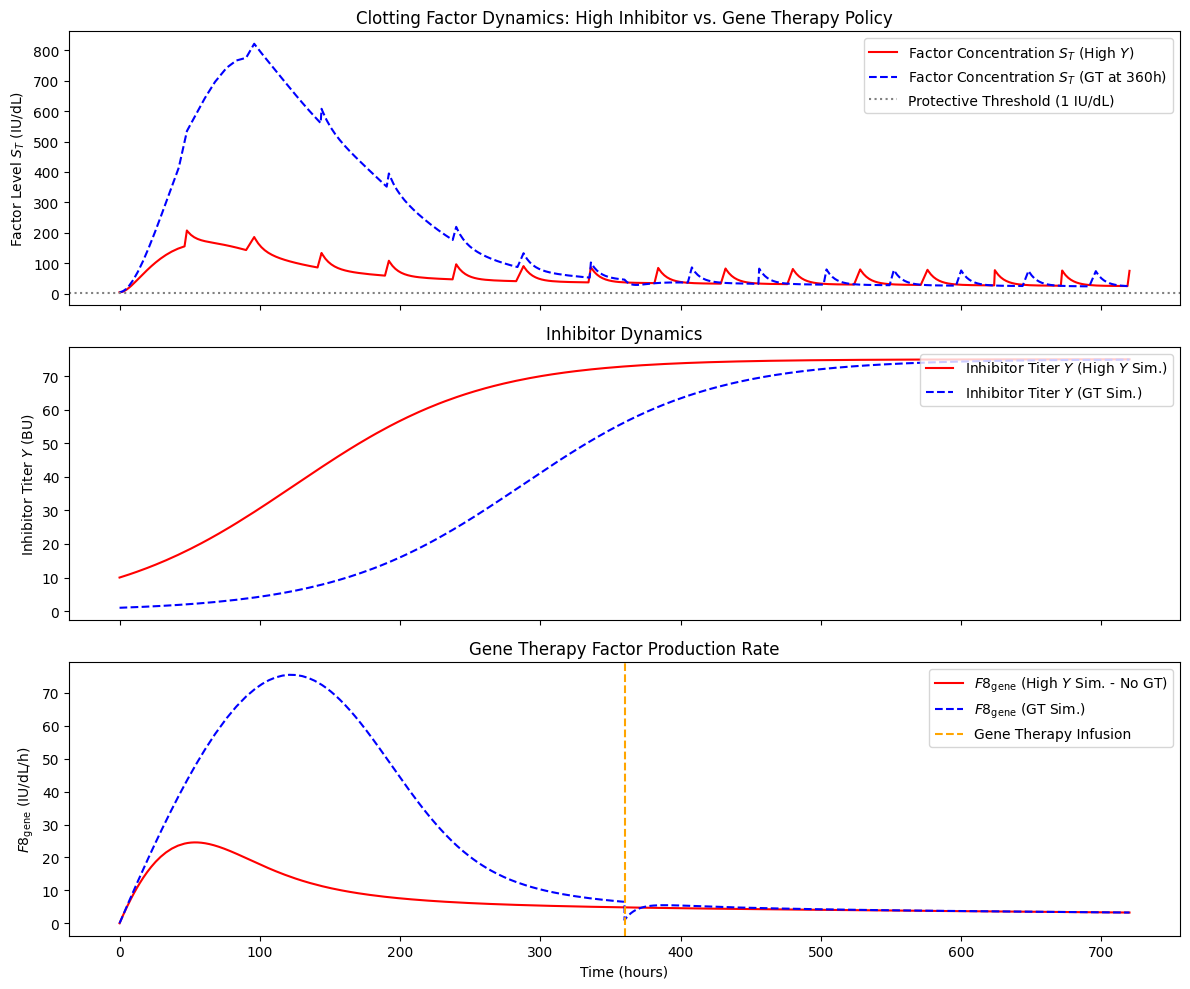
\includegraphics[width=\textwidth]{Figures/clotting_dynamics.png}
\caption{Illustrative clotting-factor dynamics under two policies. Top:
factor activity $S_T$ for a high-inhibitor infusion policy (solid) and a
gene-therapy policy (dashed) that switches to infusion at $t=360$~h. Middle:
inhibitor titre. Bottom: gene-therapy production rate. Simulated illustration,
not empirical results. Figure-generation code is not included in this archive.}
\label{fig:clotting_dynamics}
\end{figure}

\section{Summary}
\label{sec:C_summary}
Specialising the general framework to haemophilia gives a factor-kinetic model
whose small-titre limit is the classical linear model
(Proposition~\ref{prop:C_linear}), whose fixed point is stable
(Proposition~\ref{prop:C_stability}), and which exhibits a clinically meaningful
inhibitor threshold (Proposition~\ref{prop:C_threshold}); immune tolerance
induction has an extinction condition (Proposition~\ref{prop:C_iti}) and gene
therapy a closed-form equilibrium (Proposition~\ref{prop:C_gt}).

Three of these results carry a threshold: the titre at which a regimen stops
protecting, the suppression at which ITI succeeds rather than nearly succeeds,
and the inhibitor level at which gene therapy becomes uneconomic. Each is a
point at which a small change in circumstance produces a large change in
outcome, and each depends on something a health system controls rather than
something the patient's biology decides. That is the connection back to the
main argument: Mr~B's Systemic Burdens domain is not a background variable in
this model, it sits inside the equations that determine whether his treatment
works.

The eleven tests in \texttt{verification/tests/test\_haemophilia.py} assert
these results, together with the worked examples above: the steady states at
each titre, the point at which the regimen stops protecting, and the critical
suppression for immune tolerance induction. One of them asserts that a request
for a threshold under a regimen that cannot reach protection raises an error
rather than returning a number, because a silent wrong answer is the failure
mode that matters here. The computational methods are collected in
Appendix~\ref{app:computation} and the run record in
Appendix~\ref{app:verification}.
